\documentclass[11pt,a4paper]{article}
\usepackage[T1]{fontenc}
\usepackage[utf8]{inputenc}
\usepackage[spanish,es-nodecimaldot,es-noshorthands]{babel}
\usepackage{lmodern}
\usepackage[margin=2.5cm]{geometry}
\usepackage{graphicx}
\usepackage{booktabs}
\usepackage{tabularx}
\usepackage{longtable}
\usepackage{array}
\usepackage{xcolor}
\usepackage{listings}
\usepackage{tikz}
\usetikzlibrary{positioning,arrows.meta}
\usepackage{caption}
\usepackage[hidelinks]{hyperref}

\graphicspath{{figs/}}
\captionsetup{font=small,labelfont=bf}
\setlength{\parskip}{0.5em}
\setlength{\parindent}{0pt}
\newcolumntype{Y}{>{\raggedright\arraybackslash}X}

\definecolor{codigofondo}{HTML}{F5F5F3}
\lstset{
  basicstyle=\ttfamily\footnotesize,
  backgroundcolor=\color{codigofondo},
  frame=single, rulecolor=\color{black!20},
  breaklines=true, showstringspaces=false,
  columns=fullflexible, keepspaces=true,
  aboveskip=0.8em, belowskip=0.8em
}

% Marca visible para lo que falta completar antes de la entrega.
\newcommand{\pendiente}[1]{\par\noindent\fcolorbox{red!70!black}{red!6}{\parbox{\dimexpr\linewidth-2\fboxsep-2\fboxrule}{\small\textbf{Pendiente antes de entregar:} #1}}\par}

\newcommand{\sarn}{sARN}
\newcommand{\dG}{$\Delta G$}
\newcommand{\codigo}[1]{\texttt{\detokenize{#1}}}

\title{\textbf{Descifrando la lógica de los sARN bacterianos:\\ determinantes de unión a ARNm, chaperonas y RNasa E}\\[0.6em]
\large Informe final --- Proyecto interno de la UNSAM\\ Licenciatura en Ciencia de Datos}
\author{Martin Ezequiel Groisman\\[0.2em] \small Responsable del proyecto: Dr. Andrés Garriz\\ \small Proyecto BACTO-RNA (UNSAM INVESTIGA, Edición 2025, código 209/25)}
\date{Noviembre de 2026}

\begin{document}
\maketitle

\begin{abstract}
\noindent
Este informe describe el trabajo realizado sobre la base de datos de interacciones entre ARN pequeños bacterianos (sARN) y sus ARN blanco del proyecto BACTO-RNA. Una tabla plana de 32.677 filas y 52 columnas se transformó en un modelo relacional de 24 tablas, con cada inconsistencia registrada, y se amplió con 17 publicaciones hasta alcanzar 63.979 interacciones y 100.839 evidencias en 49 especies. Se implementó además una búsqueda bibliográfica sistemática y reproducible, que identificó 913 trabajos candidatos, y un análisis exploratorio de la base. La energía de hibridación se recalculó para 62.571 evidencias, lo que permitió verificar los valores del compendio y mostrar que la energía sin corregir depende del largo de las ventanas y no es comparable entre técnicas. Los análisis previstos sobre chaperonas y RNasa E y la tabla de variables para reentrenamiento no se completaron: el informe detalla esas brechas y sus causas.
\end{abstract}

\tableofcontents
\newpage

%======================================================================
\section{Objetivos originales planteados}

Los objetivos se transcriben del Plan de Trabajo (Anexo II).

\textbf{Pregunta de investigación / problema abordado.} Las interacciones sARN--ARNm funcionales presentan firmas identificables en su secuencia y estructura, incluyendo regiones de reconocimiento por chaperonas (Hfq/ProQ) y sitios de procesamiento por RNasa E, que pueden extraerse mediante el análisis bioinformático y mejorar los modelos de diseño de sARN.

\textbf{Objetivo general.} Curar, ampliar y analizar la base de datos de interacciones sARN--ARNm del proyecto BACTO-RNA para caracterizar los determinantes de unión, reconocimiento por chaperonas y procesamiento por RNasa E.

\textbf{Objetivos específicos.}
\begin{enumerate}
  \item Curar, normalizar y desduplicar la base actual (más de 32.000 interacciones) e incorporar datos publicados recientemente.
  \item Caracterizar las regiones asociadas al reconocimiento por chaperonas (Hfq/ProQ) en sARN y ARNm.
  \item Identificar sitios y patrones de procesamiento por RNasa E vinculados a la interacción.
  \item Describir las propiedades de la unión sARN--ARNm (\dG, longitud, complementariedad, ubicación relativa) y generar variables para el reentrenamiento de los modelos predictivos.
\end{enumerate}

\textbf{Productos esperados.} Un conjunto de datos curado, ampliado y anotado de interacciones sARN--ARNm; una tabla de variables biológicamente informativas (chaperonas, RNasa E, termodinámica y estructura); y un informe reproducible que alimente el reentrenamiento de los modelos predictivos de diseño de sARN.

%======================================================================
\section{Desarrollo del trabajo}

\subsection{Contexto y estado del arte}

Las enfermedades bacterianas de las plantas disponen de pocas herramientas de control, limitadas a compuestos cúpricos y antibióticos poco específicos. El proyecto BACTO-RNA explora como alternativa el silenciamiento génico antibacteriano mediante ARN diseñados. Su insumo primario es una base propia de interacciones con soporte experimental, que alimenta un sistema de aprendizaje automático para predecir sitios de interacción y generar sARN optimizados.

Los sARN regulan la expresión génica a nivel postranscripcional, apareándose con ARN mensajeros y modificando su traducción o su estabilidad \cite{hor2020}. La complementariedad no alcanza para explicar qué interacciones ocurren. La chaperona Hfq estabiliza a los sARN y favorece el apareamiento \cite{vogel2011}; ProQ, otra proteína de unión a ARN, reconoce ARN por su estructura \cite{holmqvist2018} y puede competir con Hfq o complementarla \cite{melamed2020}. La RNasa E, por su parte, inicia la degradación de numerosos transcriptos \cite{bandyra2018}, y su mapa global de cortes se describió en \emph{Salmonella} \cite{chao2017}.

La mayor parte de los datos de la base proviene de métodos de alto rendimiento que capturan los dos ARN de un par en una misma molécula híbrida. RIL-seq liga los ARN que coinmunoprecipitan con Hfq \cite{melamed2016}; CLASH captura los híbridos unidos a una proteína entrecruzada, como la RNasa E \cite{waters2017}; y GRIL-seq los liga en la célula sin purificar una proteína \cite{han2016}. Cada técnica informa algo distinto: la región que cubren las lecturas, la hélice exacta o un enriquecimiento. Comprender esa diferencia a partir de los artículos fue un requisito para integrar los datos y es un tema recurrente de este informe.

Para predecir la hibridación se usan herramientas basadas en el modelo termodinámico del plegado, como el paquete ViennaRNA \cite{lorenz2011} e IntaRNA, que incorpora la accesibilidad del sitio y la presencia de una región semilla \cite{busch2008,mann2017}.

\subsection{Actividades realizadas y rol del estudiante}

El estudiante tuvo a su cargo el diseño del modelo de datos, la definición de los criterios de depuración e integración, el desarrollo de los procesos de carga, la búsqueda bibliográfica, el análisis exploratorio y la validación de los resultados, bajo la dirección del Dr. Andrés Garriz.

Las actividades se organizaron en cinco etapas:
\begin{enumerate}
  \item Auditoría y normalización de la tabla plana original a un modelo relacional.
  \item Incorporación de Gebhardt et al.\ 2023 \cite{gebhardt2023}, trabajada directamente desde el artículo y sus datos suplementarios, como patrón de carga para fuentes futuras.
  \item Diseño e implementación de la búsqueda sistemática de interacciones publicadas desde 2022.
  \item Integración de un compendio de interacciones elaborado por el Dr.\ Garriz fuera del repositorio, en un esquema distinto.
  \item Análisis exploratorio de la base resultante y recálculo de energías de hibridación.
\end{enumerate}

\textbf{Autoría de los datos.} El compendio de la etapa 4, incluidos los dúplex predichos y las regiones semilla consenso que se analizan más adelante, fue elaborado por el Dr.\ Garriz. La contribución del estudiante en ese punto fue la verificación e integración de esos datos a la base.

\textbf{Uso de inteligencia artificial.} Se utilizó un asistente de IA (Claude, de Anthropic) como apoyo para la programación y la redacción, lo que consta en la coautoría de parte de los registros del repositorio. El diseño del trabajo, los criterios adoptados y la validación de los resultados estuvieron a cargo del estudiante.

\subsection{Herramientas y metodología}

El trabajo se realizó en Python, con SQLite como motor de la base y Git/GitHub para el control de versiones. Los procesos de carga emplean únicamente la biblioteca estándar, de modo que la base se puede regenerar sin instalar dependencias. Las herramientas bioinformáticas se ejecutan en contenedores de BioContainers con versión fija (ViennaRNA 2.7.2 e IntaRNA 3.4.1).

Se adoptaron cuatro principios de trabajo:
\begin{itemize}
  \item \textbf{Determinismo.} Ante los mismos datos de entrada se obtienen los mismos identificadores.
  \item \textbf{Trazabilidad.} Cada evidencia remite a su fila de origen y cada corrección consta en la tabla \codigo{qc_issue}. Cada carga deja una bitácora con las filas por tabla antes y después y el SHA-1 de sus fuentes.
  \item \textbf{Idempotencia.} Los cargadores se pueden volver a correr sin duplicar datos.
  \item \textbf{Pruebas de punta a punta.} Una prueba copia el repositorio a un directorio limpio, corre la cadena completa y comprueba que los archivos versionados se regeneren idénticos.
\end{itemize}
Estos principios responden también a los criterios FAIR para la gestión de datos científicos \cite{wilkinson2016}.

\subsection{Arquitectura de la solución}

La Figura~\ref{fig:cadena} resume la cadena de procesamiento. La base se reconstruye desde el archivo original, cada fuente nueva se agrega con su propio cargador, y la lista de exclusión que resulta alimenta la búsqueda de trabajos que aún no están incorporados.

\begin{figure}[htbp]
\centering
\begin{tikzpicture}[
  caja/.style={draw=black!55, rounded corners=2pt, fill=#1, align=center, font=\scriptsize, minimum height=9mm, text width=33mm},
  caja/.default=white,
  flecha/.style={-{Stealth[length=2mm]}, draw=black!60}, node distance=7mm and 8mm]
\node[caja=black!6] (csv) {Tabla plana\\32.677 $\times$ 52};
\node[caja=blue!8, right=of csv] (build) {\texttt{build\_db.py}\\normalización};
\node[caja=black!6, right=of build] (bd) {Base SQLite\\24 tablas, 2 vistas};
\node[caja=black!6, above=of build] (fuentes) {Gebhardt 2023 y\\compendio Garriz};
\node[caja=blue!8, right=of fuentes] (load) {\texttt{load\_*.py}\\cargadores};
\node[caja=blue!8, below=of bd] (excl) {\texttt{exportar\_exclusion.py}};
\node[caja=blue!8, left=of excl] (busq) {\texttt{buscar\_candidatos.py}\\PubMed, Europe PMC};
\node[caja=black!6, left=of busq] (cand) {913 candidatos\\para cribado};
\node[caja=blue!8, below=of excl, text width=33mm] (dg) {\texttt{recalcular\_dg.py}\\Docker};
\draw[flecha] (csv)--(build); \draw[flecha] (build)--(bd);
\draw[flecha] (fuentes)--(load); \draw[flecha] (load)--(bd);
\draw[flecha] (bd)--(excl); \draw[flecha] (excl)--(busq); \draw[flecha] (busq)--(cand);
\draw[flecha] (bd.east)-- ++(4mm,0) |- (dg.east);
\end{tikzpicture}
\caption{Cadena de procesamiento. En azul, los programas; en gris, los datos.}
\label{fig:cadena}
\end{figure}

\subsubsection{Modelo de datos}

La tabla plana repetía en cada fila la cepa, las moléculas, la secuencia y la bibliografía. El modelo relacional \cite{codd1970} guarda cada entidad una sola vez y recompone la información mediante claves (Figura~\ref{fig:modelo}). Las tablas se organizan en cinco bloques: origen biológico, moléculas, interacción, bibliografía y control de calidad.

\begin{figure}[htbp]
\centering
\begin{tikzpicture}[
  t/.style={draw=black!55, rounded corners=2pt, fill=#1, font=\footnotesize\ttfamily, minimum height=7mm, minimum width=25mm},
  t/.default=black!5,
  r/.style={-{Stealth[length=2mm]}, draw=black!60}, node distance=6mm and 7mm]
\node[t] (species) {species};
\node[t, right=of species] (strain) {strain};
\node[t, right=of strain] (genome) {genome};
\node[t, right=of genome] (replicon) {replicon};
\node[t=blue!10, below=of strain] (rna) {rna};
\node[t=blue!10, below=of genome] (interaction) {interaction};
\node[t, left=of rna] (seq) {sequence};
\node[t=blue!10, below=of interaction] (evidence) {interaction\_evidence};
\node[t, left=of evidence, xshift=-6mm] (site) {binding\_site};
\node[t, right=of evidence, xshift=2mm] (study) {study};
\node[t, right=of study, xshift=-3mm] (pub) {publication};
\node[t, below=of evidence] (stats) {evidence\_stats};
\node[t, left=of stats] (duplex) {duplex\_prediction};
\draw[r] (species)--(strain); \draw[r] (strain)--(genome); \draw[r] (genome)--(replicon);
\draw[r] (strain)--(rna); \draw[r] (genome)--(interaction); \draw[r] (rna)--(interaction);
\draw[r] (rna)--(seq); \draw[r] (interaction)--(evidence); \draw[r] (evidence)--(site);
\draw[r] (evidence)--(study); \draw[r] (study)--(pub); \draw[r] (evidence)--(stats);
\draw[r] (evidence.south west)--(duplex.north east);
\end{tikzpicture}
\caption{Principales tablas del modelo. Las flechas indican la dependencia entre entidades; se omiten las tablas auxiliares.}
\label{fig:modelo}
\end{figure}

La decisión central fue separar el par biológico de la evidencia que lo respalda. Una interacción es única por genoma y una evidencia corresponde a cada registro experimental. Así, las 32.538 filas depuradas del archivo original se reducen a 29.656 pares sin perder evidencia. El esquema impone esa unicidad:

\begin{lstlisting}[language=SQL]
CREATE TABLE interaction (
  interaction_id TEXT PRIMARY KEY,
  genome_id      TEXT NOT NULL REFERENCES genome(genome_id),
  srna_rna_id    TEXT NOT NULL REFERENCES rna(rna_id),
  target_rna_id  TEXT NOT NULL REFERENCES rna(rna_id),
  is_self_interaction INTEGER NOT NULL DEFAULT 0,
  UNIQUE (genome_id, srna_rna_id, target_rna_id)
);
\end{lstlisting}

Otras dos decisiones de diseño:
\begin{itemize}
  \item Los sARN y los blancos comparten la tabla \codigo{rna}, porque un mismo ARN puede cumplir ambos roles. En la base final, 1.337 moléculas actúan como regulador y como blanco.
  \item La molécula (\codigo{rna_id}, una por cepa) y la secuencia (\codigo{seq_id}, un hash SHA-1 del contenido) son entidades independientes, relacionadas por una tabla intermedia. Una molécula puede tener varias secuencias registradas (690 casos) y una secuencia puede corresponder a varias moléculas (209 casos).
\end{itemize}

\subsection{Resultados}

\subsubsection{Normalización de la base}

La auditoría detectó inconsistencias en 153.088 celdas. Las más frecuentes (Tabla~\ref{tab:qc}) derivan de que el archivo pasó por una planilla de cálculo en español. Dos situaciones se conservaron sin corregir por no existir un criterio confiable sin recurrir a la fuente primaria: la longitud declarada del sARN difiere de la secuencia en 1.374 filas, y la extensión derivada de las coordenadas difiere de la secuencia en 18.066 sitios de unión. Ambas constan en \codigo{qc_issue}.

\begin{table}[htbp]
\centering\small
\caption{Principales inconsistencias del archivo original.}
\label{tab:qc}
\begin{tabularx}{\linewidth}{Y r Y}
\toprule
Tipo & Casos & Tratamiento\\
\midrule
Booleanos de Excel en español (\texttt{FALSO}, \texttt{VERDADERO}) & 87.476 & Conversión a 0/1\\
Marcadores de nulo (\texttt{NA}, \texttt{\#N/D}, \texttt{None}) & 39.869 & Conversión a nulo efectivo\\
Extensión de coordenadas distinta de la secuencia & 18.066 & Conservado y registrado\\
Citas bibliográficas en una columna numérica & 3.063 & Traslado a \texttt{publication}; recuento recalculado\\
Longitud declarada distinta de la secuencia & 1.374 & Conservado y registrado\\
Hebra inválida & 171 & Anulación\\
Filas duplicadas exactas & 139 & Eliminación\\
Fragmentos de JSON en la columna de \dG{} & 73 & Depuración\\
\bottomrule
\end{tabularx}
\end{table}

\subsubsection{Ampliación de la base}

La Tabla~\ref{tab:ampliacion} muestra la evolución de la base. La carga de Gebhardt et al.\ 2023 aportó 1.484 evidencias de RIL-seq y validaciones en \emph{P. aeruginosa} PAO1. El compendio aportó 66.817 evidencias de 16 publicaciones de 2022 a 2026 y tres especies nuevas: \emph{Acinetobacter baumannii}, \emph{Clostridioides difficile} y \emph{Bordetella pertussis}. De sus 58 estudios posteriores a la migración se cargaron 44; se excluyeron las reingestas de trabajos ya presentes y un estudio de CLIP-seq sin pares ARN--ARN, y también 223 filas en las que una molécula pertenecía al fago lambda.

\begin{table}[htbp]
\centering\small
\caption{Magnitudes de la base al normalizar y al final de las incorporaciones.}
\label{tab:ampliacion}
\begin{tabular}{l r r}
\toprule
Magnitud & Normalización & Base final\\
\midrule
Interacciones únicas (sARN $\rightarrow$ blanco) & 29.656 & 63.979\\
Evidencias & 32.538 & 100.839\\
Moléculas de ARN & 14.027 & 29.634\\
Secuencias únicas & 32.744 & 102.685\\
Sitios de unión & 35.813 & 160.935\\
Publicaciones & 112 & 129\\
Especies / cepas & 46 / 72 & 49 / 79\\
Genomas & 74 & 81\\
\bottomrule
\end{tabular}
\end{table}

\subsubsection{Búsqueda bibliográfica sistemática}

Se automatizó una búsqueda en PubMed y Europe PMC de trabajos publicados desde enero de 2022, complementada con un rastreo de las citas de las publicaciones de alto rendimiento de la base. Siguiendo la práctica de las revisiones sistemáticas \cite{page2021}, cada corrida registra fecha, consulta y resultados. La búsqueda arrojó 913 candidatos, y recuperó los 5 trabajos de 2022 y 2023 que la base ya contenía en ese momento, lo que funcionó como control de sensibilidad. Una preclasificación con expresiones regulares ordena los candidatos para el cribado (Tabla~\ref{tab:candidatos}); no reemplaza la lectura.

\begin{table}[htbp]
\centering\small
\caption{Preclasificación de los 913 candidatos.}
\label{tab:candidatos}
\begin{tabularx}{\linewidth}{c Y r}
\toprule
Prioridad & Criterio & Candidatos\\
\midrule
1 & Método directo de alto rendimiento (RIL-seq, CLASH, GRIL, LIGR) & 35\\
2 & Patógeno ESKAPE sin cobertura, con término de sARN & 72\\
3 & Otro método experimental detectado & 243\\
4 & Sin método detectado en el resumen & 372\\
7 & Probable ARN eucariota & 117\\
8 & Solo predicción computacional & 11\\
9 & Revisión, editorial u otro texto no primario & 63\\
\bottomrule
\end{tabularx}
\end{table}

\subsubsection{Análisis exploratorio}

\textbf{Cobertura.} Tres especies concentran el 76\,\% de las interacciones (Figura~\ref{fig:especies}), y 40 de las 49 especies tienen menos de 100. Entre los patógenos ESKAPE siguen sin datos \emph{Enterococcus faecium} y \emph{Enterobacter}. La base es también muy reciente: el año 2025 aporta casi la mitad de las evidencias (Figura~\ref{fig:anios}), lo que confirma el valor de la actualización.

\begin{figure}[htbp]
\centering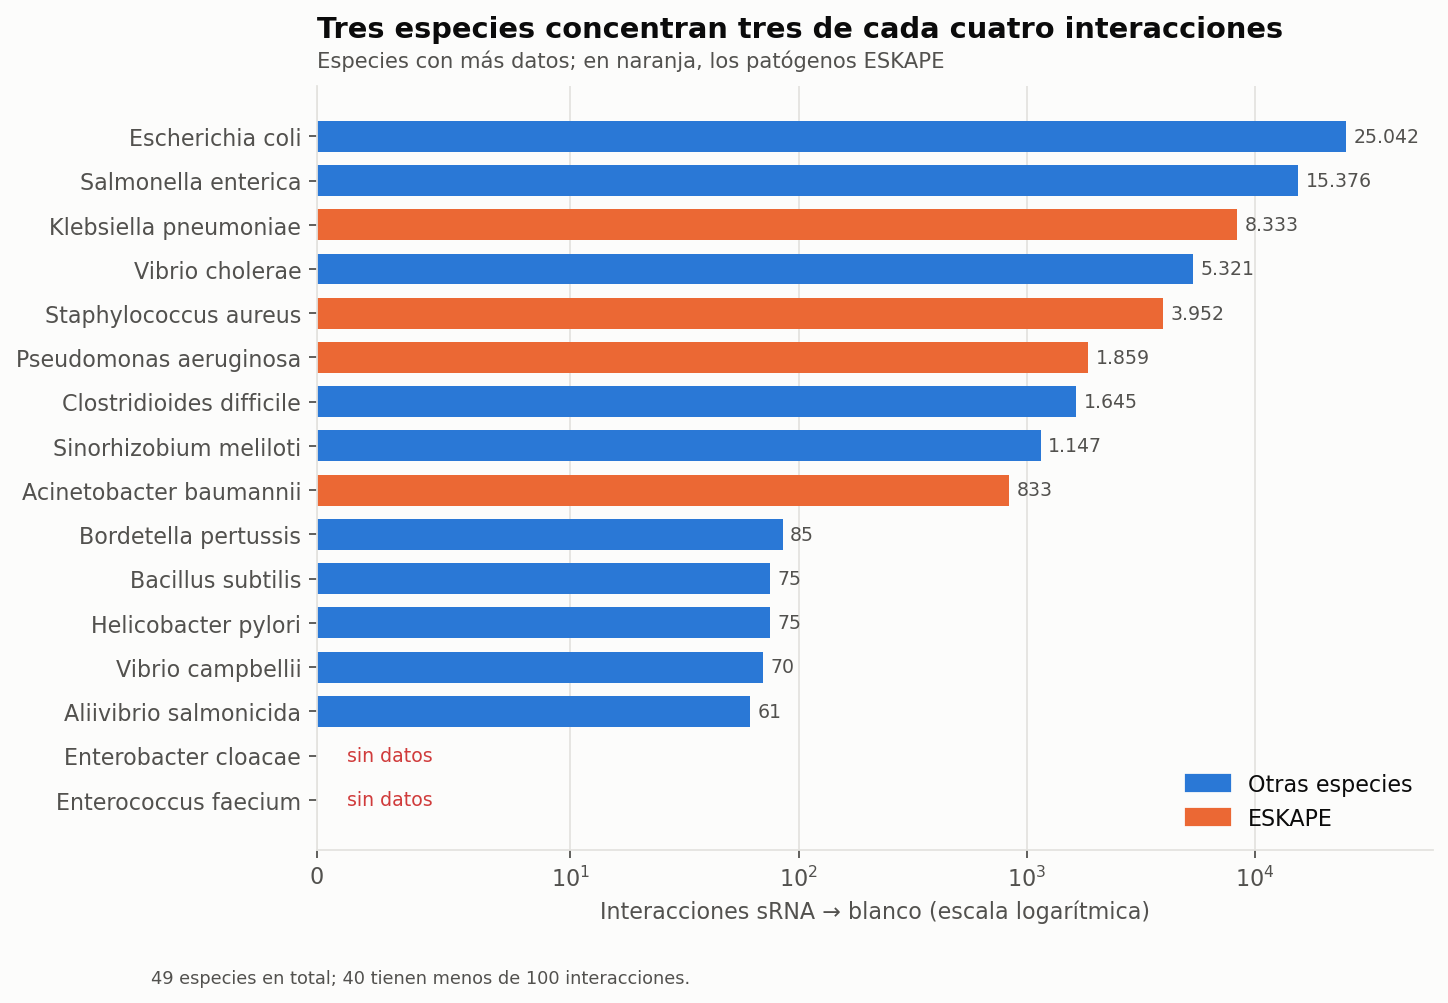
\includegraphics[width=0.82\linewidth]{01_cobertura_especies.png}
\caption{Interacciones por especie, en escala logarítmica. Los patógenos ESKAPE se destacan en naranja.}
\label{fig:especies}
\end{figure}

\begin{figure}[htbp]
\centering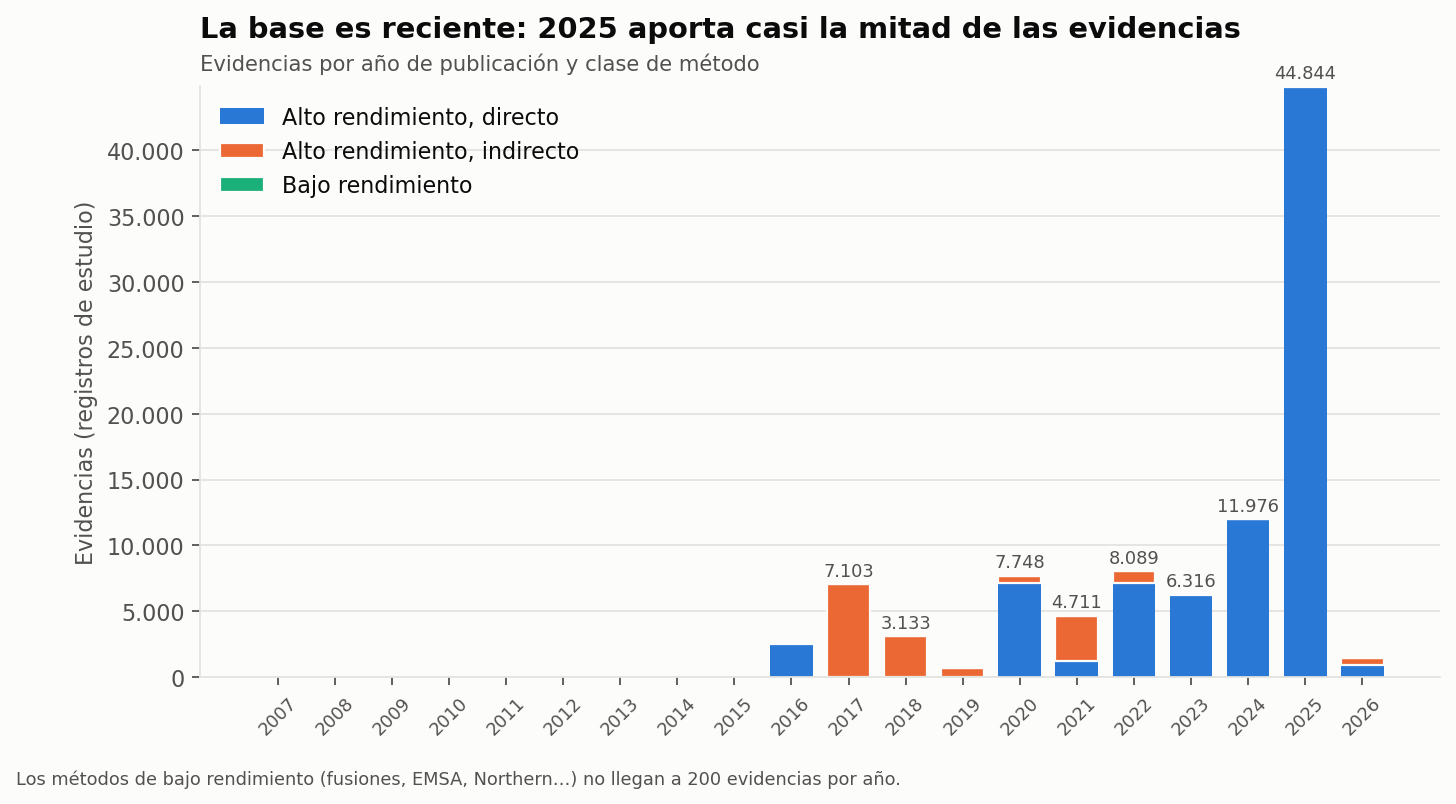
\includegraphics[width=0.82\linewidth]{02_evidencias_por_anio.png}
\caption{Evidencias por año de publicación y clase de método.}
\label{fig:anios}
\end{figure}

\textbf{Técnicas.} RIL-seq con Hfq domina los datos (Figura~\ref{fig:tecnicas}). El panel derecho advierte de un problema de integración: en CLASH con RNasa III, el 82\,\% de los pares tiene como \emph{regulador} un ARN que no es un sARN. Esos pares no deberían entrar sin filtro a un modelo de diseño de sARN.

\begin{figure}[htbp]
\centering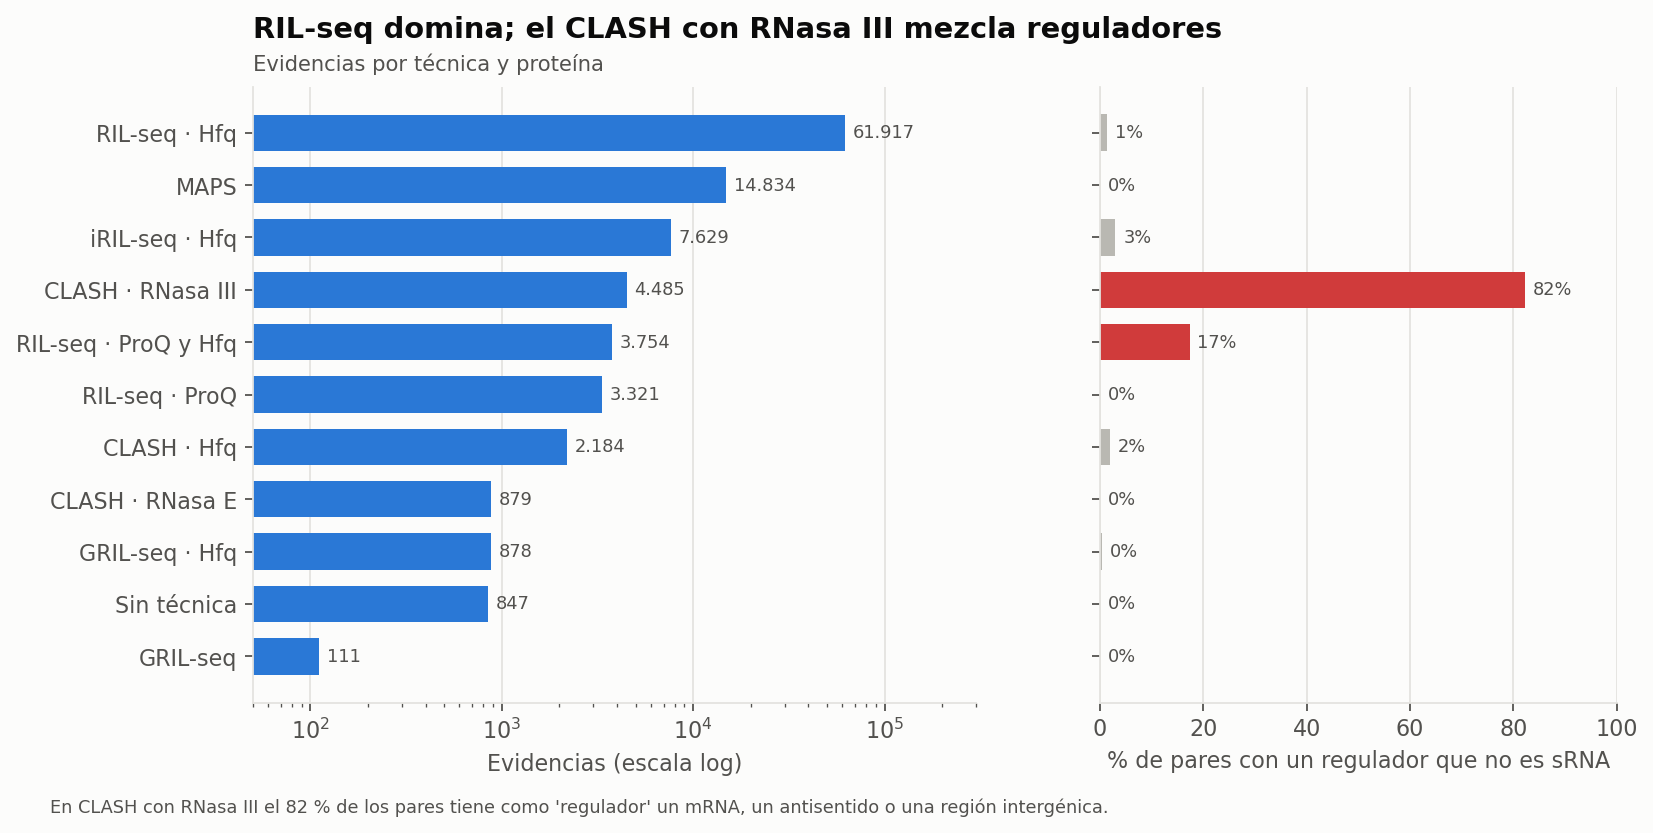
\includegraphics[width=0.88\linewidth]{03_tecnicas.png}
\caption{Evidencias por técnica y proteína, y porcentaje de pares cuyo regulador no es un sARN.}
\label{fig:tecnicas}
\end{figure}

\textbf{Respaldo.} El 91,5\,\% de los pares fue informado por una sola publicación (Figura~\ref{fig:respaldo}). Dos trabajos sobre \emph{E. coli} con al menos 500 pares comparten, como máximo, un índice de Jaccard de 0,27, y los valores más altos corresponden a trabajos del mismo laboratorio. La red es además muy desigual: de los 1.448 sARN reguladores, 396 tienen un único blanco y 9 superan los mil. Estos resultados aconsejan cautela al tomar la ausencia de un par como evidencia negativa.

\begin{figure}[htbp]
\centering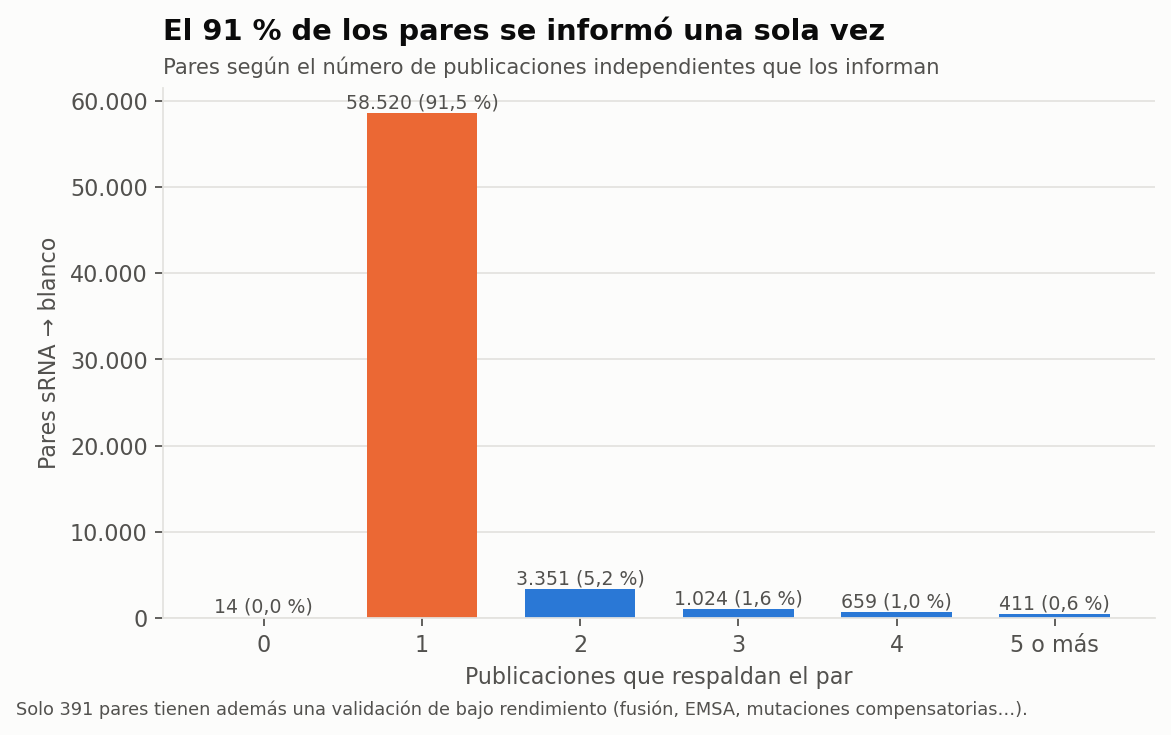
\includegraphics[width=0.72\linewidth]{06_respaldo_por_publicaciones.png}
\caption{Pares sARN--blanco según el número de publicaciones que los informan.}
\label{fig:respaldo}
\end{figure}

\textbf{Dúplex frente a un modelo nulo.} La Figura~\ref{fig:duplex} compara el \dG{} predicho por el compendio con el de secuencias barajadas conservando dinucleótidos. En CLASH con Hfq la señal es muy clara (mediana de $-11{,}2$~kcal/mol respecto del nulo), mientras que en RIL-seq con Hfq casi desaparece ($-0{,}8$~kcal/mol). La interpretación, coherente con la descripción de los métodos en la literatura, es que RIL-seq informa la región que cubren las lecturas y no el sitio de apareamiento: una ventana más larga diluye la señal. Es una observación con consecuencias directas para el reentrenamiento, porque indica que las ventanas de distintas técnicas no son intercambiables.

\begin{figure}[htbp]
\centering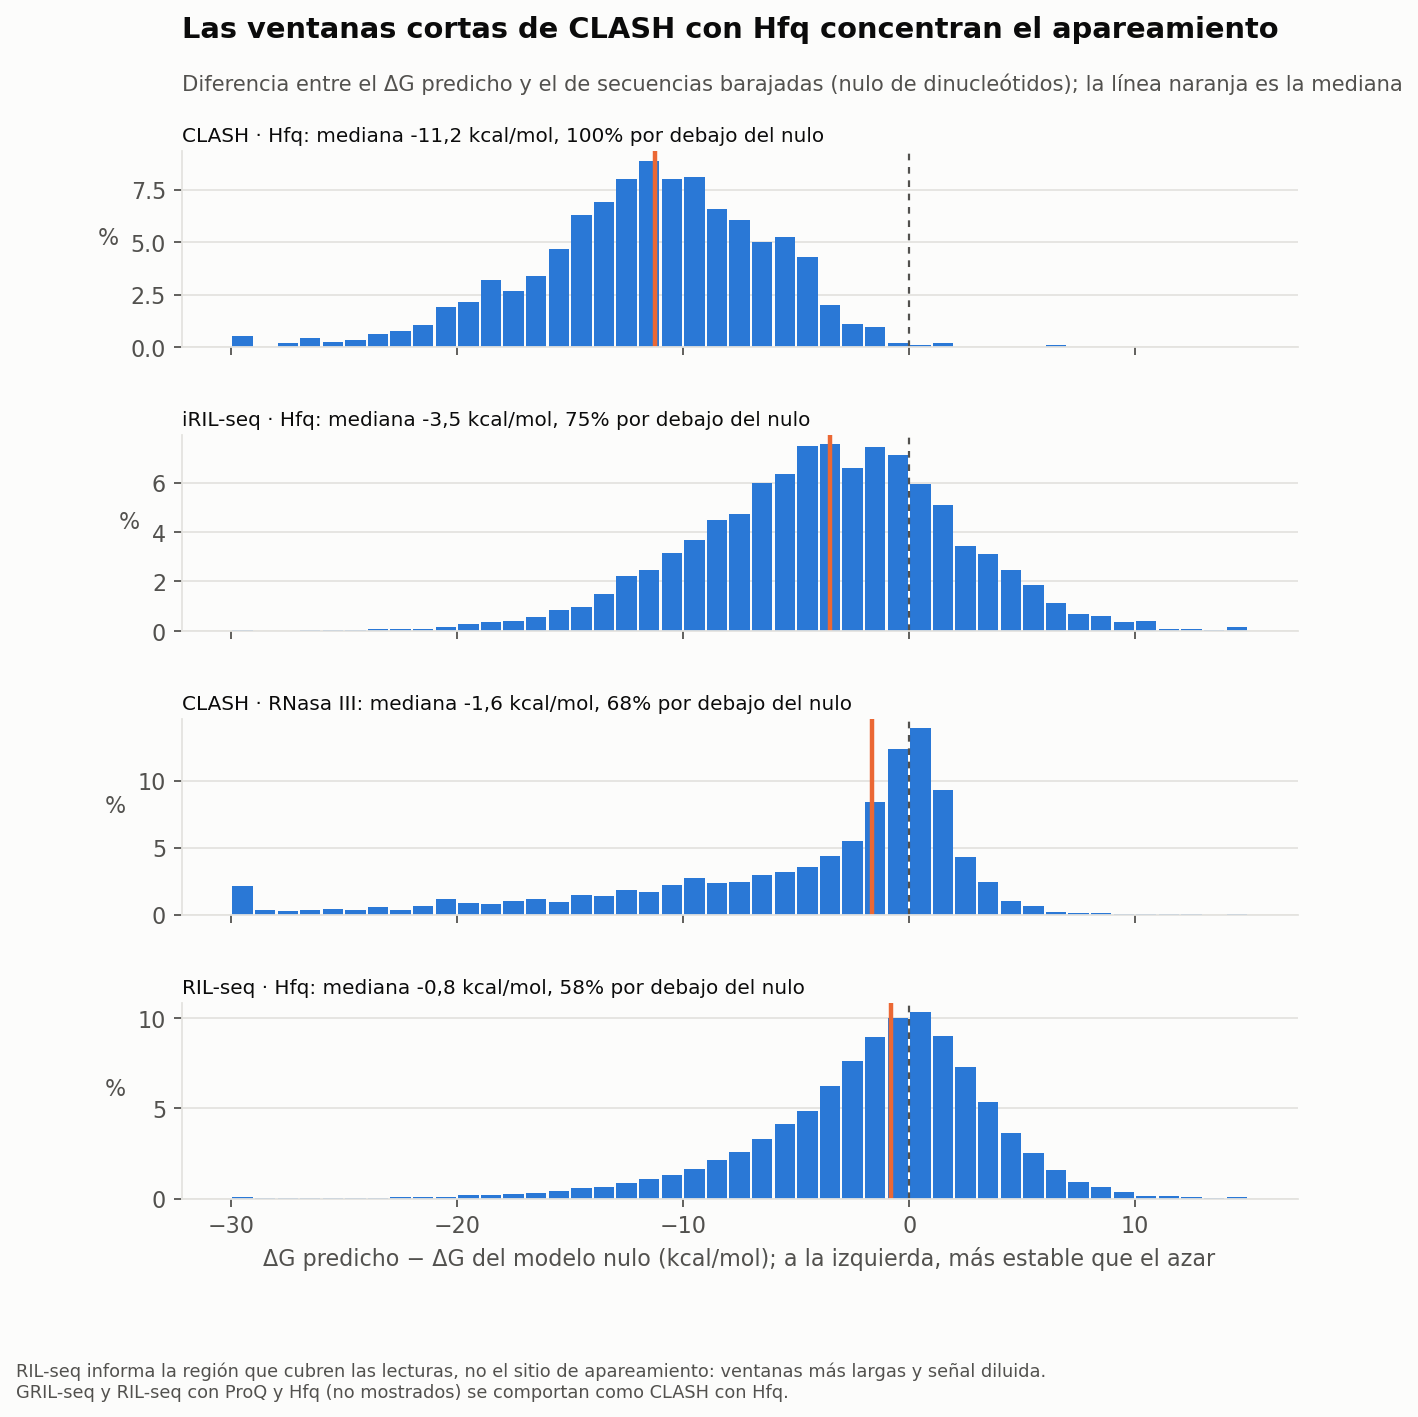
\includegraphics[width=0.72\linewidth]{08_duplex_vs_nulo.png}
\caption{Diferencia entre el \dG{} predicho y el del modelo nulo de dinucleótidos, según técnica.}
\label{fig:duplex}
\end{figure}

\textbf{Regiones semilla.} De las 84 regiones consenso del compendio, 21 resultan significativas ($q<0{,}05$). Aunque suele describirse el extremo 5$'$ como región de apareamiento, aquí se reparten entre ese extremo y la mitad 3$'$ del sARN (Figura~\ref{fig:semillas}). Dado el número reducido de casos, se trata de una observación descriptiva.

\begin{figure}[htbp]
\centering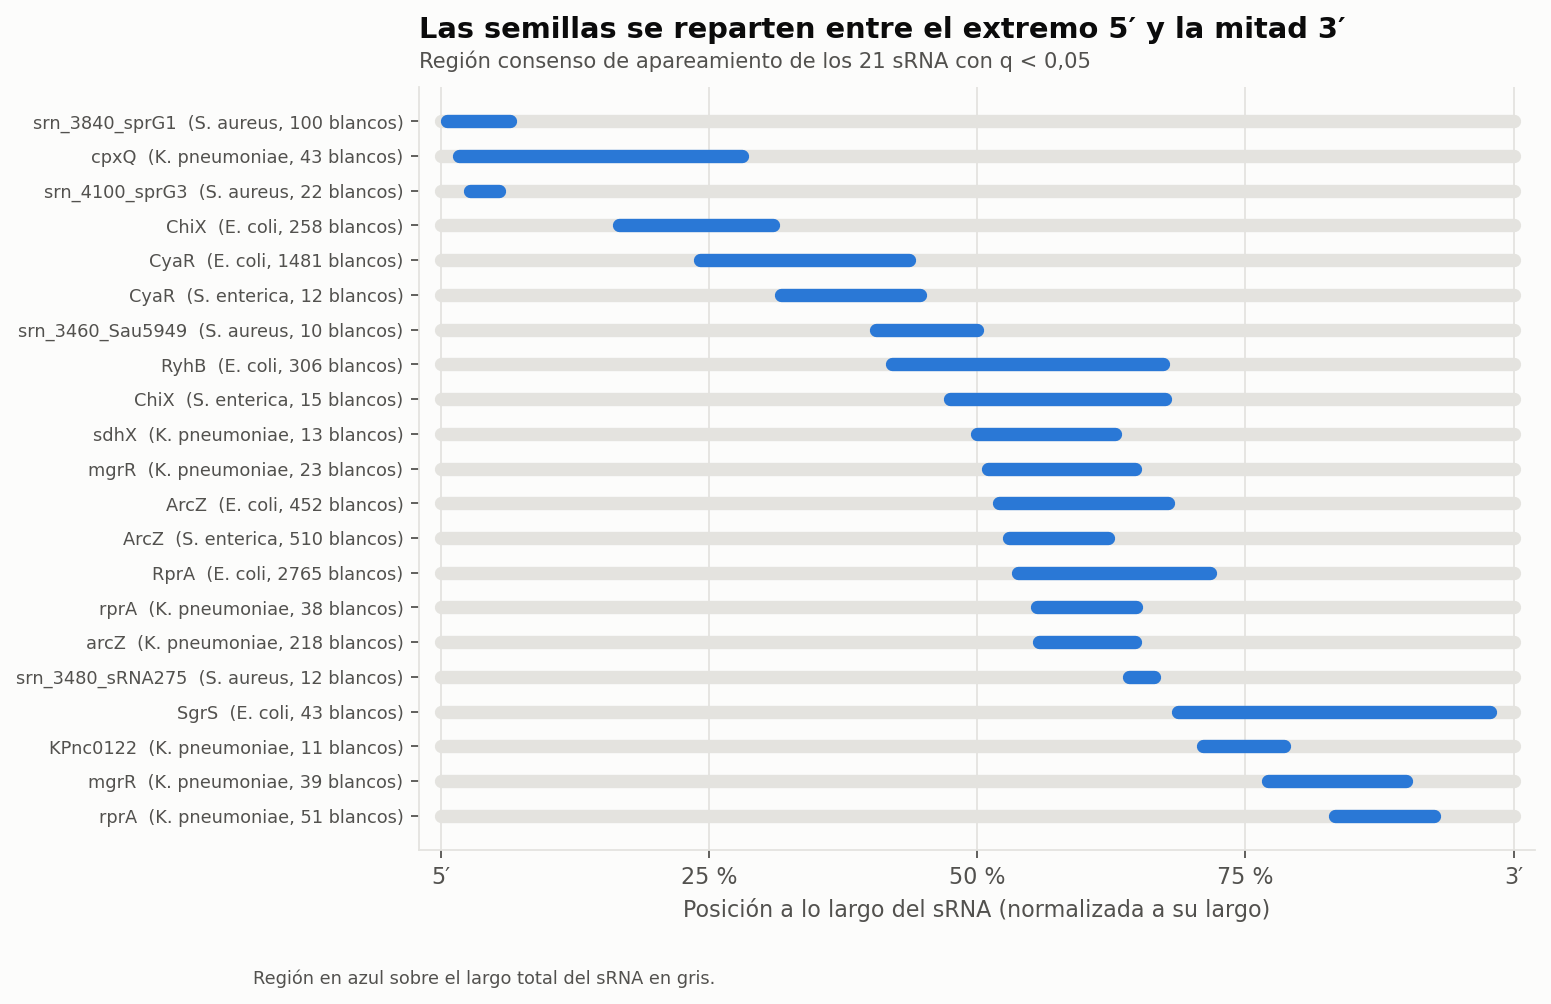
\includegraphics[width=0.82\linewidth]{09_regiones_semilla.png}
\caption{Región consenso de apareamiento de los 21 sARN con $q<0{,}05$, sobre el largo normalizado de cada sARN.}
\label{fig:semillas}
\end{figure}

\textbf{Composición y región del blanco.} Los sARN tienen menor contenido de GC que los ARNm de su especie, con una diferencia mayor en los genomas ricos en GC (Figura~\ref{fig:gc}). En cuanto a la región del blanco, la mitad de las evidencias no la informa, y entre las que sí lo hacen predomina la región codificante (Figura~\ref{fig:region}). Esa falta de información es una limitación para el objetivo de describir la ubicación relativa de la unión.

\begin{figure}[htbp]
\centering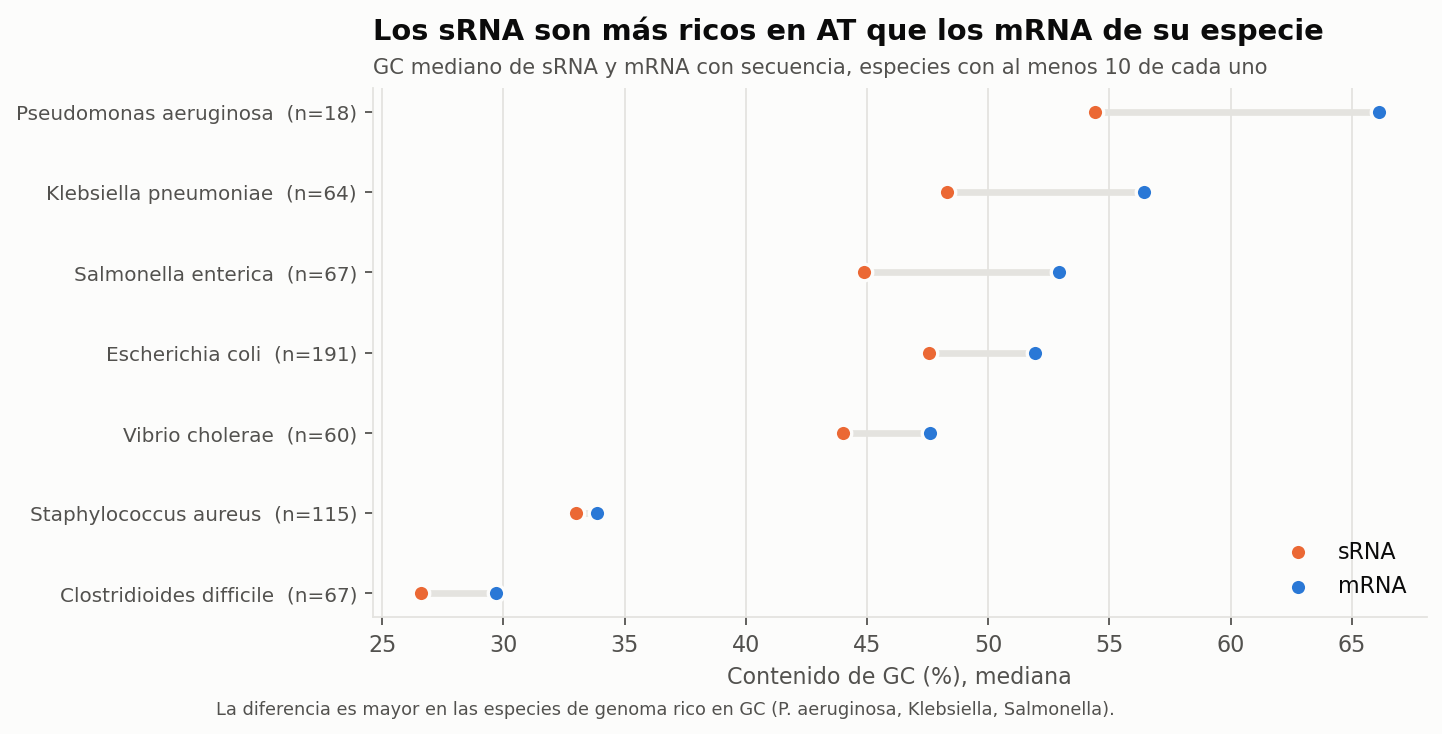
\includegraphics[width=0.80\linewidth]{10_gc_srna_vs_mrna.png}
\caption{Contenido de GC mediano de sARN y ARNm por especie.}
\label{fig:gc}
\end{figure}

\begin{figure}[htbp]
\centering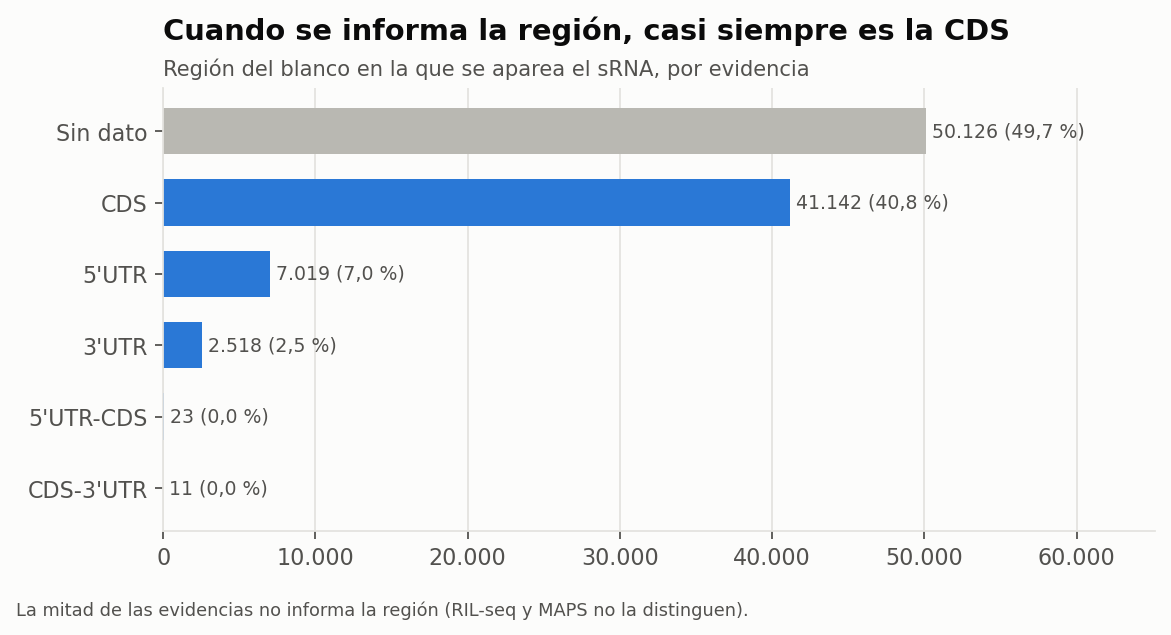
\includegraphics[width=0.68\linewidth]{11_region_del_blanco.png}
\caption{Región del blanco en la que se aparea el sARN, por evidencia.}
\label{fig:region}
\end{figure}

\textbf{Calidad residual.} La Figura~\ref{fig:calidad} reúne los problemas que siguen presentes y que quien analice la base debe considerar, junto con las correcciones más frecuentes.

\begin{figure}[htbp]
\centering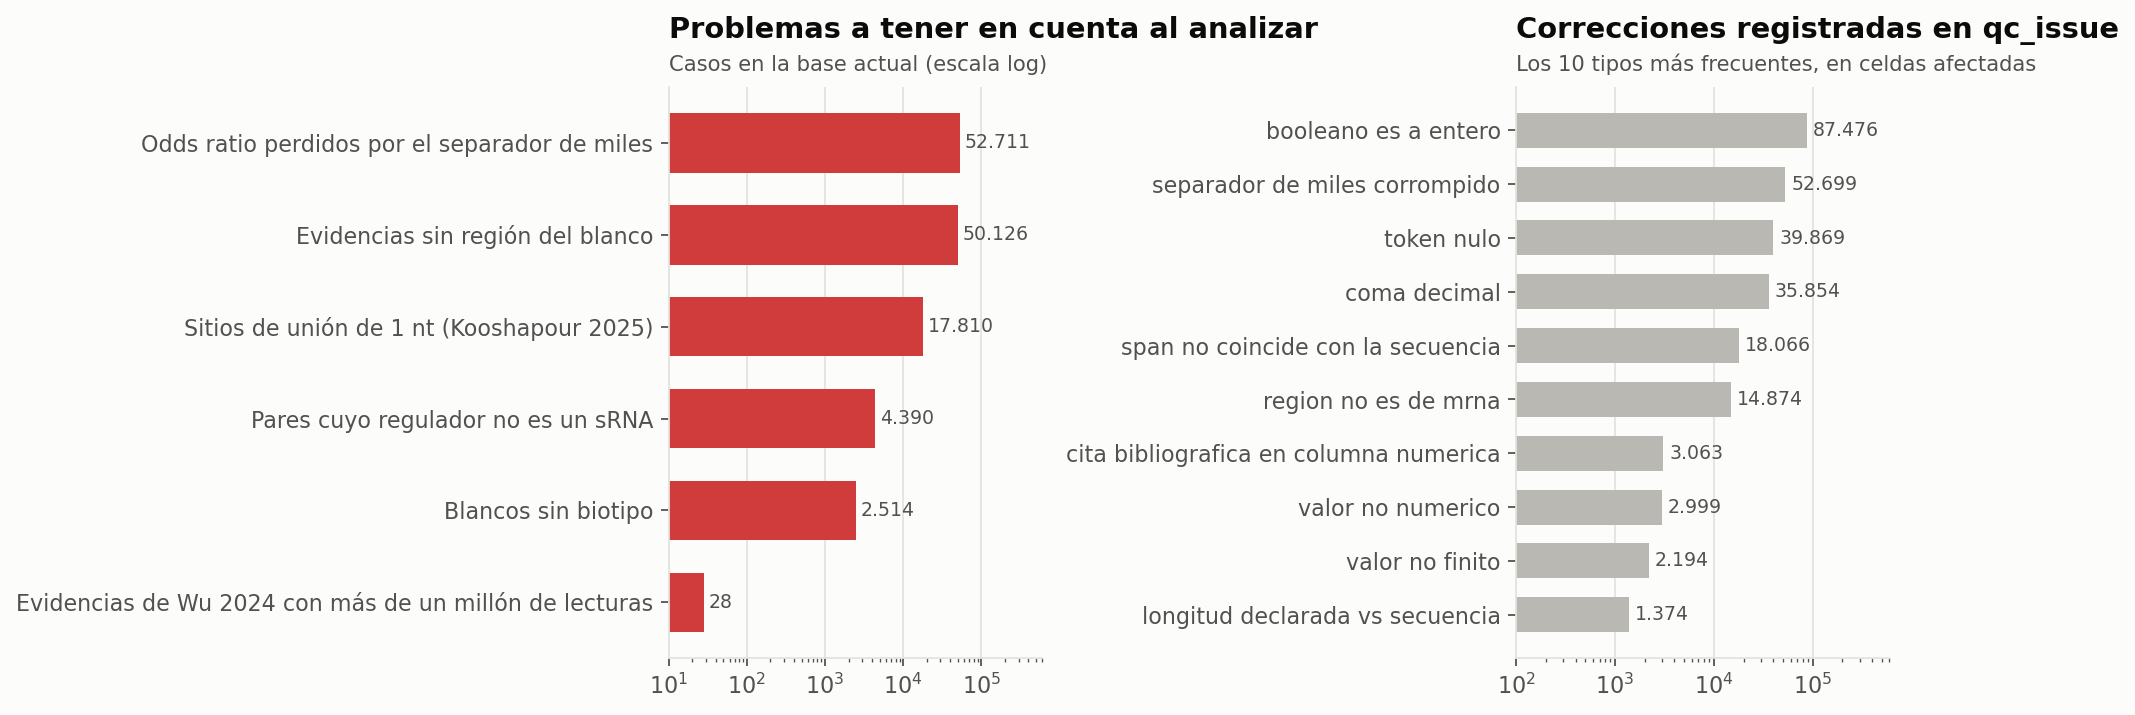
\includegraphics[width=\linewidth]{12_calidad_de_datos.png}
\caption{Problemas vigentes en la base (izquierda) y tipos de corrección registrados (derecha), en escala logarítmica.}
\label{fig:calidad}
\end{figure}

\subsubsection{Recálculo de la energía de hibridación}
\label{sec:dg}

La base contiene dos fuentes de \dG{}: el valor del archivo original, cuyo método no está documentado, y el de los dúplex del compendio. Para verificarlos se implementó \codigo{scripts/recalcular_dg.py}, que recalcula cada par con ventanas de secuencia disponibles mediante tres enfoques: RNAduplex (solo apareamiento intermolecular), RNAcofold junto con RNAfold (energía del complejo respecto de cada ventana plegada por separado) e IntaRNA (hibridación con accesibilidad y semilla).

De las 100.839 evidencias, 77.445 tienen ambas ventanas de secuencia. Las secuencias, almacenadas en alfabeto de ADN, se convierten a ARN. Se excluyen las ventanas de menos de 7 nucleótidos (la longitud de semilla por defecto de IntaRNA y un indicio de error de coordenadas) y los pares que suman más de 1.000 nucleótidos, por el costo cúbico de RNAcofold. Cada par distinto se calcula una sola vez, y cada evidencia excluida queda marcada con su motivo en \codigo{db/analisis/dg_recalculado.csv}, una tabla con una fila por evidencia. El resultado cubre 62.571 evidencias (Tabla~\ref{tab:cobertura}), correspondientes a 59.974 pares distintos de secuencias. IntaRNA, con su semilla por defecto, devolvió una predicción para 46.116 de ellas (73,7\,\%).

\begin{table}[htbp]
\centering\small
\caption{Cobertura del recálculo de la energía de hibridación.}
\label{tab:cobertura}
\begin{tabular}{l r}
\toprule
Estado & Evidencias\\
\midrule
Calculadas & 62.571\\
Sin alguna de las dos ventanas de secuencia & 23.394\\
Ventana de menos de 7 nucleótidos & 14.849\\
Pares de más de 1.000 nucleótidos & 25\\
\midrule
Total & 100.839\\
\bottomrule
\end{tabular}
\end{table}

\textbf{Procedencia de los valores existentes.} El \dG{} de los dúplex del compendio coincide con RNAduplex (ViennaRNA 2.7.2, 37\,°C) en la totalidad de las 46.353 evidencias comparables, lo que verifica esos valores e identifica el método con el que se calcularon. El \dG{} del archivo original, en cambio, coincide con RNAduplex solo en el 15,7\,\% de las 20.058 evidencias comparables, y es en mediana 7,31~kcal/mol menos negativo. La coincidencia se concentra en una técnica: alcanza el 99,2\,\% en CLASH con RNasa III y no supera el 1\,\% en ninguna de las demás (Tabla~\ref{tab:dgtecnica}). La columna original reúne por lo tanto valores de procedencia heterogénea y no debería usarse como una única variable.

\textbf{Dependencia del largo de la ventana.} La Figura~\ref{fig:dglargo} muestra que el \dG{} de RNAduplex se vuelve más negativo cuanto más larga es la ventana (correlación de Spearman $\rho=-0{,}55$ en el conjunto y entre $-0{,}41$ y $-0{,}94$ dentro de cada técnica). Es esperable, porque una ventana más larga ofrece más oportunidades de apareamiento y este método no considera el plegado de cada molécula. La energía neta de RNAcofold, que descuenta el plegado de cada ventana, e IntaRNA, que incorpora la accesibilidad, dependen menos del largo: dentro de cada técnica, $\rho$ va de $-0{,}08$ a $-0{,}73$ en la primera y de $+0{,}07$ a $-0{,}66$ en la segunda.

\begin{figure}[htbp]
\centering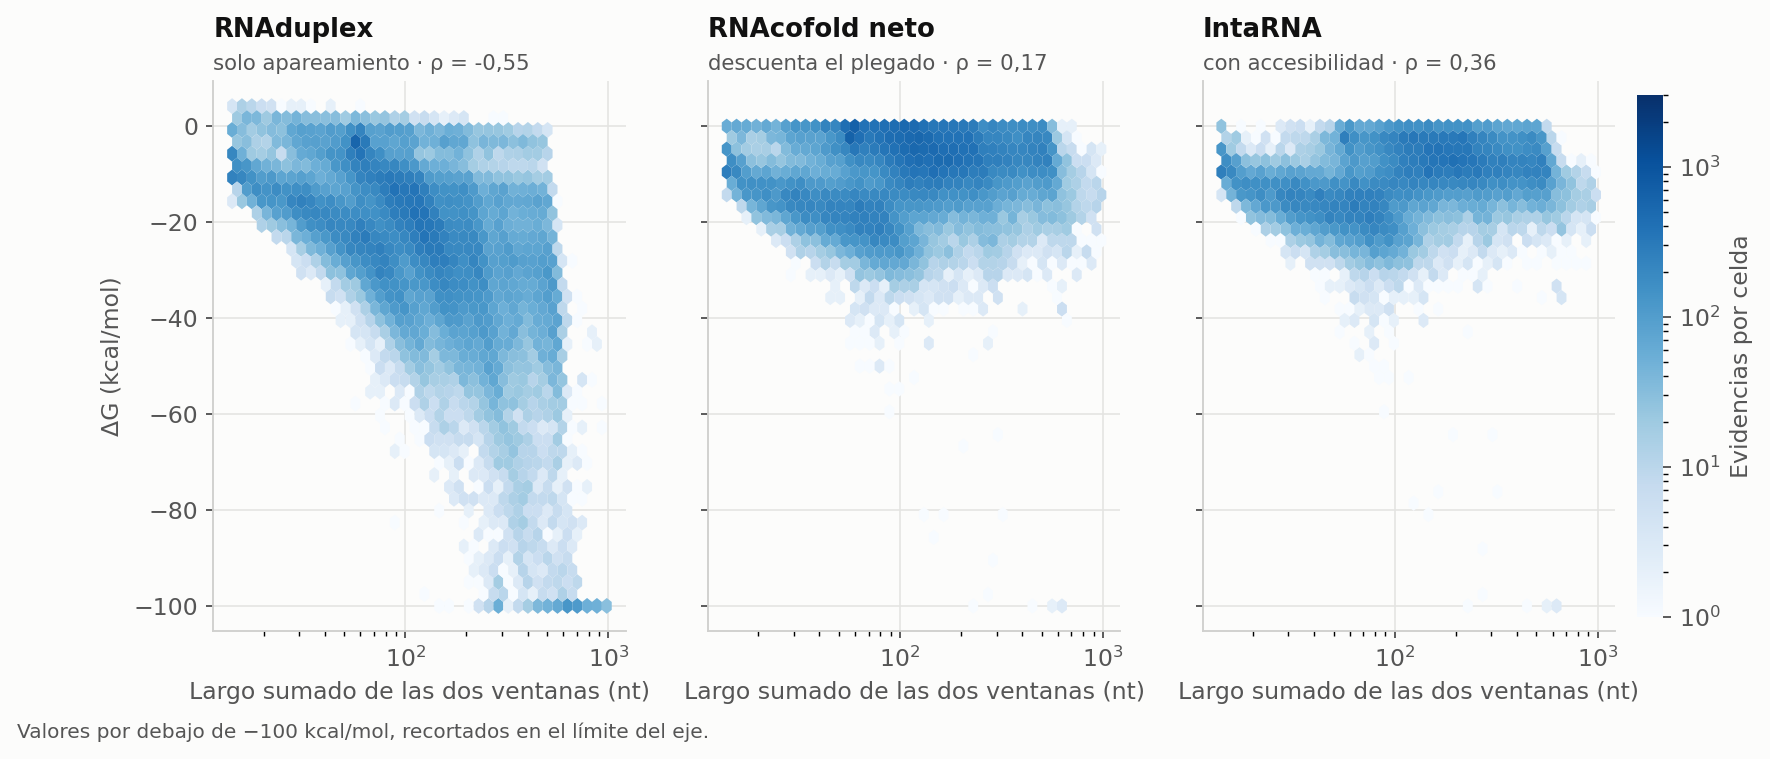
\includegraphics[width=\linewidth]{13_dg_segun_largo_ventana.png}
\caption{Energía de hibridación según el largo sumado de las dos ventanas, para los tres enfoques. El color indica el número de evidencias en cada celda.}
\label{fig:dglargo}
\end{figure}

\begin{table}[htbp]
\centering\small
\caption{Medianas de la energía (kcal/mol) y del largo de las ventanas (nt) por técnica, y porcentaje de evidencias cuyo \dG{} original coincide con RNAduplex. Se omiten las técnicas con menos de 500 evidencias.}
\label{tab:dgtecnica}
\begin{tabular}{l r r r r r r}
\toprule
Técnica & Evid. & Largo sARN/blanco & RNAduplex & Cofold neto & IntaRNA & Coinc.\ (\%)\\
\midrule
RIL-seq con Hfq & 35.989 & 37 / 96 & $-20{,}0$ & $-5{,}1$ & $-7{,}1$ & 0,0\\
Purificación por afinidad MS2 & 8.552 & 27 / 25 & $-20{,}6$ & $-16{,}8$ & $-15{,}5$ & 0,3\\
iRIL-seq con Hfq & 6.895 & 60 / 77 & $-29{,}9$ & $-10{,}3$ & $-9{,}5$ & ---\\
CLASH con RNasa III & 4.467 & 36 / 39 & $-10{,}9$ & $-5{,}5$ & $-9{,}5$ & 99,2\\
RIL-seq con ProQ y Hfq & 3.309 & 22 / 22 & $-20{,}5$ & $-16{,}7$ & $-16{,}3$ & 0,3\\
CLASH con Hfq & 1.959 & 18 / 18 & $-18{,}3$ & $-15{,}7$ & $-14{,}8$ & 0,5\\
GRIL-seq con Hfq & 599 & 36 / 36 & $-29{,}0$ & $-22{,}4$ & $-20{,}4$ & 0,0\\
CLASH con RNasa E & 520 & 31 / 31 & $-19{,}0$ & $-13{,}4$ & $-13{,}3$ & 0,8\\
\bottomrule
\end{tabular}
\end{table}

Esto refuerza la observación de la Figura~\ref{fig:duplex}: las técnicas informan ventanas de largos muy distintos, de modo que una energía sin corregir no es comparable entre ellas. Para el reentrenamiento conviene usar la energía neta o la de IntaRNA, e incorporar la técnica y el largo de las ventanas como variables. La salida de IntaRNA y RNAcofold debe interpretarse con una salvedad: al calcularse sobre las ventanas, ignora el contexto del transcripto completo.

\subsection{Problemas y desafíos técnicos}

\begin{table}[htbp]
\centering\small
\caption{Principales desafíos y su resolución.}
\label{tab:desafios}
\begin{tabularx}{\linewidth}{>{\raggedright\arraybackslash}p{0.42\linewidth} Y}
\toprule
Desafío & Abordaje\\
\midrule
Distinta capitalización de nombres entre lotes (\texttt{RyhB}, \texttt{ryhB}) & Clave de comparación normalizada que conserva la denominación original\\
Mismos genes con distintos identificadores (\texttt{PA\#\#\#\#}, \texttt{PA14\_\#\#\#\#\#}) & Búsqueda por locus, BioCyc, nombre y sinónimos, en la cepa de cada estudio\\
Coordenadas que mezclan marcos genómicos y relativos & Campo \texttt{coord\_frame} estimado por heurística, documentado como tal\\
\emph{Odds ratio} sin coma decimal en la fuente (\texttt{144.852.081.396.333}) & Valor irrecuperable: queda nulo y consta en \texttt{qc\_issue}\\
DOI erróneos y autores mal escritos en la fuente & Corrección desde PubMed, Crossref y las series de GEO citadas\\
Valores $p$ de un suplemento repetidos por error de copia & Detección al leer el material suplementario; se usó la hoja de significativos de los autores\\
Redes intermitentes en las API bibliográficas (HTTP 503) & Reintentos con registro del error; la búsqueda se puede reanudar\\
\bottomrule
\end{tabularx}
\end{table}

%======================================================================
\section{Ajustes y diferencias respecto de lo previsto}

El objetivo específico 1 se cumplió en su mayor parte, y el 4 de forma parcial. Los objetivos 2 y 3 no se completaron. La Tabla~\ref{tab:brechas} compara cada actividad del cronograma con lo efectivamente realizado.

{\small
\begin{longtable}{>{\raggedright\arraybackslash}p{0.34\linewidth} >{\raggedright\arraybackslash}p{0.14\linewidth} >{\raggedright\arraybackslash}p{0.44\linewidth}}
\caption{Actividades previstas y estado final.}\label{tab:brechas}\\
\toprule
Actividad prevista & Estado & Detalle\\
\midrule\endfirsthead
\toprule
Actividad prevista & Estado & Detalle\\
\midrule\endhead
Familiarización y auditoría inicial de calidad & Realizado & Reporte de inconsistencias y tabla \texttt{qc\_issue}.\\
Curación y normalización & Realizado en lo principal & Desduplicación, hebras y modelo relacional. Las discrepancias entre coordenadas y secuencias se registraron, pero no se resolvieron.\\
Búsqueda e incorporación de interacciones recientes & Parcial & Búsqueda hecha (913 candidatos). Quedan 898 sin cribar y faltan las bases curadas por especie. Se incorporaron 17 publicaciones, 16 de ellas desde el compendio.\\
Recuperación y control de secuencias desde NCBI & Parcial & Se recuperaron metadatos bibliográficos y genómicos. No se contrastaron las secuencias contra los genomas de referencia.\\
Cálculo y verificación de parámetros termodinámicos & Realizado en lo principal & \dG{} recalculado para 62.571 evidencias con tres enfoques (sección~\ref{sec:dg}). No se utilizó RNAup ni se calcularon descriptores estructurales adicionales.\\
Caracterización de regiones de Hfq/ProQ & No realizado & Sin catálogo de motivos. Solo hay anotaciones de origen: proteína del estudio, clase de Hfq en 64 moléculas y regiones semilla del compendio.\\
Identificación de sitios de RNasa E & No realizado & Sin mapa de sitios. La base dispone de 879 evidencias de CLASH con RNasa E, aún sin analizar con ese fin.\\
Análisis de patrones y motivos & Parcial & Análisis exploratorio descriptivo. No se aplicaron \emph{clustering}, enriquecimiento ni reducción de dimensionalidad.\\
Variables y entrega del dataset & Parcial & La base curada y la tabla de \dG{} están disponibles. No se construyó la tabla integrada de variables.\\
Visualización, informe y presentación & Realizado & Figuras y presente informe.\\
\bottomrule
\end{longtable}
}

\textbf{Causas de las brechas.} El trabajo se desarrolló entre el 30 de julio y el 9 de noviembre de 2026, poco más de tres meses frente a los seis del cronograma, e insumió 135 horas, frente a las 140 previstas. La dedicación total fue, por lo tanto, cercana a la planificada, pero concentrada en la mitad del tiempo calendario y distribuida de otra manera. El trabajo se cerró antes de lo previsto para confeccionar este informe, cuya fecha de entrega es el 13 de noviembre de 2026. La mayor parte del esfuerzo se dedicó a la calidad y la integración de los datos, una tarea que el plan subestimó. Las fuentes llegaron con errores que había que entender antes de corregir, y cada una usaba identificadores y convenciones propias. Además, la incorporación del compendio, recibido el 21 de octubre de 2026, duplicó el tamaño de la base, y se priorizó integrarlo con el mismo criterio de trazabilidad antes de analizar datos que todavía estaban cambiando. Esta decisión favoreció la solidez del insumo a costa de los análisis biológicos.

\textbf{Ajustes metodológicos.} El plan preveía notebooks con pandas y NumPy, y Biopython para acceder a NCBI. Los procesos de carga se implementaron en cambio como programas de Python con la biblioteca estándar y consultas directas a las API, lo que facilita regenerar la base de punta a punta. El plan mencionaba también RNAup, que no se utilizó: el recálculo se apoya en RNAduplex, RNAcofold e IntaRNA.

\textbf{Limitaciones.}
\begin{itemize}
  \item Persiste el sesgo hacia organismos modelo, que el plan ya identificaba como riesgo. La base casi no contiene especies fitopatógenas, que son el destino final del proyecto.
  \item Los datos sobre ProQ y RNasa E son escasos: solo 599 y 520 evidencias, respectivamente, tienen sus ventanas de secuencia, por lo que su análisis será exploratorio.
  \item Las figuras del análisis exploratorio se generaron de forma separada y el programa que las produce aún no está versionado en el repositorio.
  \item Los hallazgos son descriptivos y no permiten inferencias causales.
\end{itemize}

\textbf{Trabajo futuro.} Por orden de prioridad: completar el cribado de los candidatos de prioridad 1 y 2; contrastar las coordenadas y secuencias contra los genomas de referencia; caracterizar las regiones de Hfq/ProQ y los sitios de RNasa E; y construir la tabla de variables para el reentrenamiento, separando las ventanas según la técnica.

%======================================================================
\section{Aprendizajes y vínculo con la Ciencia de Datos}

Este trabajo recorrió buena parte del ciclo de un proyecto de ciencia de datos: reunir fuentes, modelarlas, depurarlas, explorarlas y verificar los resultados. No llegó a la etapa de modelado predictivo, pero justamente por eso deja ver cuánto de lo que un modelo puede aprender se decide antes de entrenarlo.

\textbf{Los datos se entienden por cómo se generaron.} Una columna significa lo que hizo el proceso que la produjo, no lo que sugiere su nombre. La leyenda de los datos suplementarios de Gebhardt et al.\ \cite{gebhardt2023} aclara que las coordenadas delimitan las lecturas quiméricas y no el apareamiento exacto, y la comparación entre técnicas de la Figura~\ref{fig:duplex} muestra que esa diferencia tiene un efecto medible. Algo parecido ocurrió con el \dG{} del archivo original: bajo un único nombre de columna reúne valores de procedencia heterogénea, algo que solo se hizo visible al recalcularlos de forma independiente (Tabla~\ref{tab:dgtecnica}). El conocimiento del dominio no fue un complemento del análisis, sino una condición para hacerlo. La literatura orientó además la distinción entre evidencia directa e indirecta y el criterio para elegir qué ARN se considera regulador en una quimera, y la búsqueda sistemática convirtió esa consulta en un proceso repetible.

\textbf{La calidad y la integración son parte del análisis.} Estas tareas concentraron la mayor parte del esfuerzo, y no fueron un paso mecánico previo. Depurar exige decidir cuándo corregir y cuándo conservar un valor dudoso: las 18.066 discrepancias entre coordenadas y secuencias se mantuvieron porque no había un criterio confiable para resolverlas sin recurrir a la fuente primaria. Registrar cada decisión en \codigo{qc_issue} la vuelve auditable y permite revisarla más adelante. Modelar los datos implicó también definir qué es una observación: separar el par biológico de la evidencia que lo respalda permitió sumar publicaciones nuevas a pares ya existentes sin duplicarlos. Las claves foráneas y las restricciones de unicidad convirtieron errores que en una planilla pasan inadvertidos en fallas explícitas durante la carga. Esa estructura también tiene un costo: consultas más complejas, compensadas con dos vistas que entregan la información ya vinculada, y la necesidad de exportar una tabla plana para el entrenamiento de modelos.

\textbf{Qué permiten concluir los datos.} Reunir muchos registros no garantiza que sean comparables ni representativos. El 91,5\,\% de los pares fue informado por una sola publicación (Figura~\ref{fig:respaldo}), de modo que la ausencia de un par no puede tomarse sin más como un ejemplo negativo, una decisión de la que depende cualquier conjunto de entrenamiento. La energía sin corregir varía con el largo de la ventana (Figura~\ref{fig:dglargo}) y ese largo cambia según la técnica, por lo que una comparación directa entre técnicas mezcla la biología con la forma de medir. La comparación con un modelo nulo muestra, por su parte, que una magnitud solo se interpreta frente a una referencia adecuada. También hay que preguntarse si cada registro pertenece a la población de interés: en CLASH con RNasa III, el 82\,\% de los pares tiene un regulador que no es un sARN (Figura~\ref{fig:tecnicas}).

\textbf{Reproducibilidad y verificación.} Un resultado que no se puede regenerar tampoco se puede auditar. Por eso se buscó que los mismos datos de entrada produjeran los mismos identificadores, que las cargas pudieran repetirse sin duplicar datos, que las herramientas corrieran en versiones fijas y que una prueba de punta a punta regenerara los archivos versionados en un directorio limpio. La verificación también se aplicó a los resultados: la búsqueda se controló con trabajos que la base ya contenía, y el recálculo confirmó el \dG{} de los dúplex del compendio en las 46.353 evidencias comparables. Esta práctica quedó incompleta en un punto, ya que el programa que genera las figuras exploratorias aún no está versionado.

\textbf{La incertidumbre del trabajo con datos.} El Plan de Trabajo definió diez actividades con entregables en seis meses, y contrastarlo con lo realizado fue un aprendizaje en sí mismo. La estimación inicial asignó un período breve a la curación y a la búsqueda, pero el trabajo real con datos heterogéneos reveló una incertidumbre mucho mayor, algo habitual en las primeras etapas de un proyecto \cite{mcconnell2006}. El volumen y los problemas de los datos solo se conocen al trabajar con ellos, de modo que un plan debe revisarse a medida que llegan. La principal enseñanza es que convenía reestimar al recibir datos nuevos y explicitar antes qué entregables se resignarían.

\textbf{Competencias desarrolladas.} El proyecto integró modelado y limpieza de datos, programación de procesos reproducibles, consulta de API científicas, análisis exploratorio y comunicación de resultados, además de la capacidad de dialogar con un dominio ajeno a la formación de base, como la biología molecular de ARN.

\textbf{Reflexión.} La lección más importante es que la calidad de un modelo depende del conocimiento que se tiene sobre sus datos. Las advertencias que surgieron de este trabajo, como las ventanas no comparables entre técnicas o los pares cuyo regulador no es un sARN, son insumos directos para el reentrenamiento de los modelos de BACTO-RNA, y hubieran pasado inadvertidas en una tabla plana.

%======================================================================
\begin{thebibliography}{99}
\bibitem{bandyra2018} Bandyra KJ, Luisi BF. RNase E and the High-Fidelity Orchestration of RNA Metabolism. \emph{Microbiol Spectr}. 2018;6(2). doi:10.1128/microbiolspec.RWR-0008-2017.
\bibitem{busch2008} Busch A, Richter AS, Backofen R. IntaRNA: efficient prediction of bacterial sRNA targets incorporating target site accessibility and seed regions. \emph{Bioinformatics}. 2008;24(24):2849--56. doi:10.1093/bioinformatics/btn544.
\bibitem{chao2017} Chao Y, Li L, Girodat D, et al. In Vivo Cleavage Map Illuminates the Central Role of RNase E in Coding and Non-coding RNA Pathways. \emph{Mol Cell}. 2017;65(1):39--51. doi:10.1016/j.molcel.2016.11.002.
\bibitem{codd1970} Codd EF. A relational model of data for large shared data banks. \emph{Commun ACM}. 1970;13(6):377--387. doi:10.1145/362384.362685.
\bibitem{gebhardt2023} Gebhardt MJ, Farland EA, Basu P, et al. Hfq-licensed RNA-RNA interactome in \emph{Pseudomonas aeruginosa} reveals a keystone sRNA. \emph{Proc Natl Acad Sci U S A}. 2023;120(21):e2218407120. doi:10.1073/pnas.2218407120.
\bibitem{han2016} Han K, Tjaden B, Lory S. GRIL-seq provides a method for identifying direct targets of bacterial small regulatory RNA by in vivo proximity ligation. \emph{Nat Microbiol}. 2016;2:16239. doi:10.1038/nmicrobiol.2016.239.
\bibitem{holmqvist2018} Holmqvist E, Li L, Bischler T, et al. Global Maps of ProQ Binding In Vivo Reveal Target Recognition via RNA Structure and Stability Control at mRNA 3$'$ Ends. \emph{Mol Cell}. 2018;70(5):971--982.e6. doi:10.1016/j.molcel.2018.04.017.
\bibitem{hor2020} Hör J, Matera G, Vogel J, et al. Trans-Acting Small RNAs and Their Effects on Gene Expression in \emph{Escherichia coli} and \emph{Salmonella enterica}. \emph{EcoSal Plus}. 2020;9(1). doi:10.1128/ecosalplus.ESP-0030-2019.
\bibitem{lorenz2011} Lorenz R, Bernhart SH, Höner zu Siederdissen C, et al. ViennaRNA Package 2.0. \emph{Algorithms Mol Biol}. 2011;6:26. doi:10.1186/1748-7188-6-26.
\bibitem{mann2017} Mann M, Wright PR, Backofen R. IntaRNA 2.0: enhanced and customizable prediction of RNA-RNA interactions. \emph{Nucleic Acids Res}. 2017;45(W1):W435--W439. doi:10.1093/nar/gkx279.
\bibitem{mcconnell2006} McConnell S. \emph{Software Estimation: Demystifying the Black Art}. Microsoft Press; 2006.
\bibitem{melamed2016} Melamed S, Peer A, Faigenbaum-Romm R, et al. Global Mapping of Small RNA-Target Interactions in Bacteria. \emph{Mol Cell}. 2016;63(5):884--97. doi:10.1016/j.molcel.2016.07.026.
\bibitem{melamed2020} Melamed S, Adams PP, Zhang A, et al. RNA-RNA Interactomes of ProQ and Hfq Reveal Overlapping and Competing Roles. \emph{Mol Cell}. 2020;77(2):411--425.e7. doi:10.1016/j.molcel.2019.10.022.
\bibitem{page2021} Page MJ, McKenzie JE, Bossuyt PM, et al. The PRISMA 2020 statement: an updated guideline for reporting systematic reviews. \emph{BMJ}. 2021;372:n71. doi:10.1136/bmj.n71.
\bibitem{vogel2011} Vogel J, Luisi BF. Hfq and its constellation of RNA. \emph{Nat Rev Microbiol}. 2011;9(8):578--89. doi:10.1038/nrmicro2615.
\bibitem{waters2017} Waters SA, McAteer SP, Kudla G, et al. Small RNA interactome of pathogenic \emph{E. coli} revealed through crosslinking of RNase E. \emph{EMBO J}. 2017;36(3):374--387. doi:10.15252/embj.201694639.
\bibitem{wilkinson2016} Wilkinson MD, Dumontier M, Aalbersberg IJ, et al. The FAIR Guiding Principles for scientific data management and stewardship. \emph{Sci Data}. 2016;3:160018. doi:10.1038/sdata.2016.18.
\end{thebibliography}

\end{document}
